\chapter{实验结果与分析}
\label{cha:04}

本章节将对本文提出的多分支因子模型推理框架进行测试与分析,并与当前流行的推理框架Pytorch JIT和计算图推理引擎OnnxRuntime进行推理延时对比。

本章主要内容如下: 

实验环境设置:本节介绍了测试使用的样例模型以及测试所使用的软硬件环境等实验准备工作。

数据实验结果:本节将测试在上述实验环境下样例模型在多分支因子模型推理框架下的性能表现,并与Pytorch JIT\cite{paszke2019pytorchimperativestylehighperformance}和OnnxRuntime进行横向比较。
实验过程中,我们将本文提出的多分支因子模型推理框架在该实验环境下,针对实时行情的不同输入和不同推理框架进行了横向和纵向的性能比较与分析。

\section{实验环境设置}
\label{cha:041}
测试中使用的实验平台, 硬件所使用的CPU为的AMD EPYC 9654 CPU。
在测试数据方面,我们基于2021年9月30日交易日全天沪铝2505的Full Tick交易数据。
在测试模型方面上,我们仍然以\autoref{fig:models}为样例输入模型的示意图。
测试时,我们使用RDTSCP实现基于CPU指令计数器的高精度纳秒计时。 
\autoref{tab:041}中为我们测试时软硬件环境的详细配置。

\begin{table}[h] %voc table result
    \centering
    \caption{实验环境中的软硬件参数}
    \begin{tabular}{|c|c|}
        \toprule
        \textbf{类型} & 信息 \\
        \midrule
        libprotoc & 3.21.12\\
        \midrule
        Blaze & 3.5\\
        \midrule
        Pytorch & 2.1\\
        \midrule
        Onnx Runtime & 1.21.0\\
        \midrule
        Intel Oneapi & 2025.0\\
        \midrule
        CPU 型号 & AMD EPYC 9654  \\
        \midrule
        C++编译器 & GCC 13.2\\
        \midrule
        性能分析工具 & RDTSCP\\
        \midrule
        操作系统信息 & Ubuntu 24.04 LTS \\
        % \midrule
        \bottomrule
    \end{tabular}
    \label{tab:041}
\end{table}

\section{实验结果与分析}
在高频交易业务场景下,不仅仅需要考虑最大加速效果,而且应当保证在条件机制无效的情况下,附属的动态优化措施本身的执行时间对模型推理的延时影响有限。

而分支缓存机制作为一种高效的过程简化方法,我们将测试样例所得到的延时测算结果进行排序,从而综合展示分支缓存机制的加速性能和执行过程的高效。

\begin{figure}[h]
    \centering
    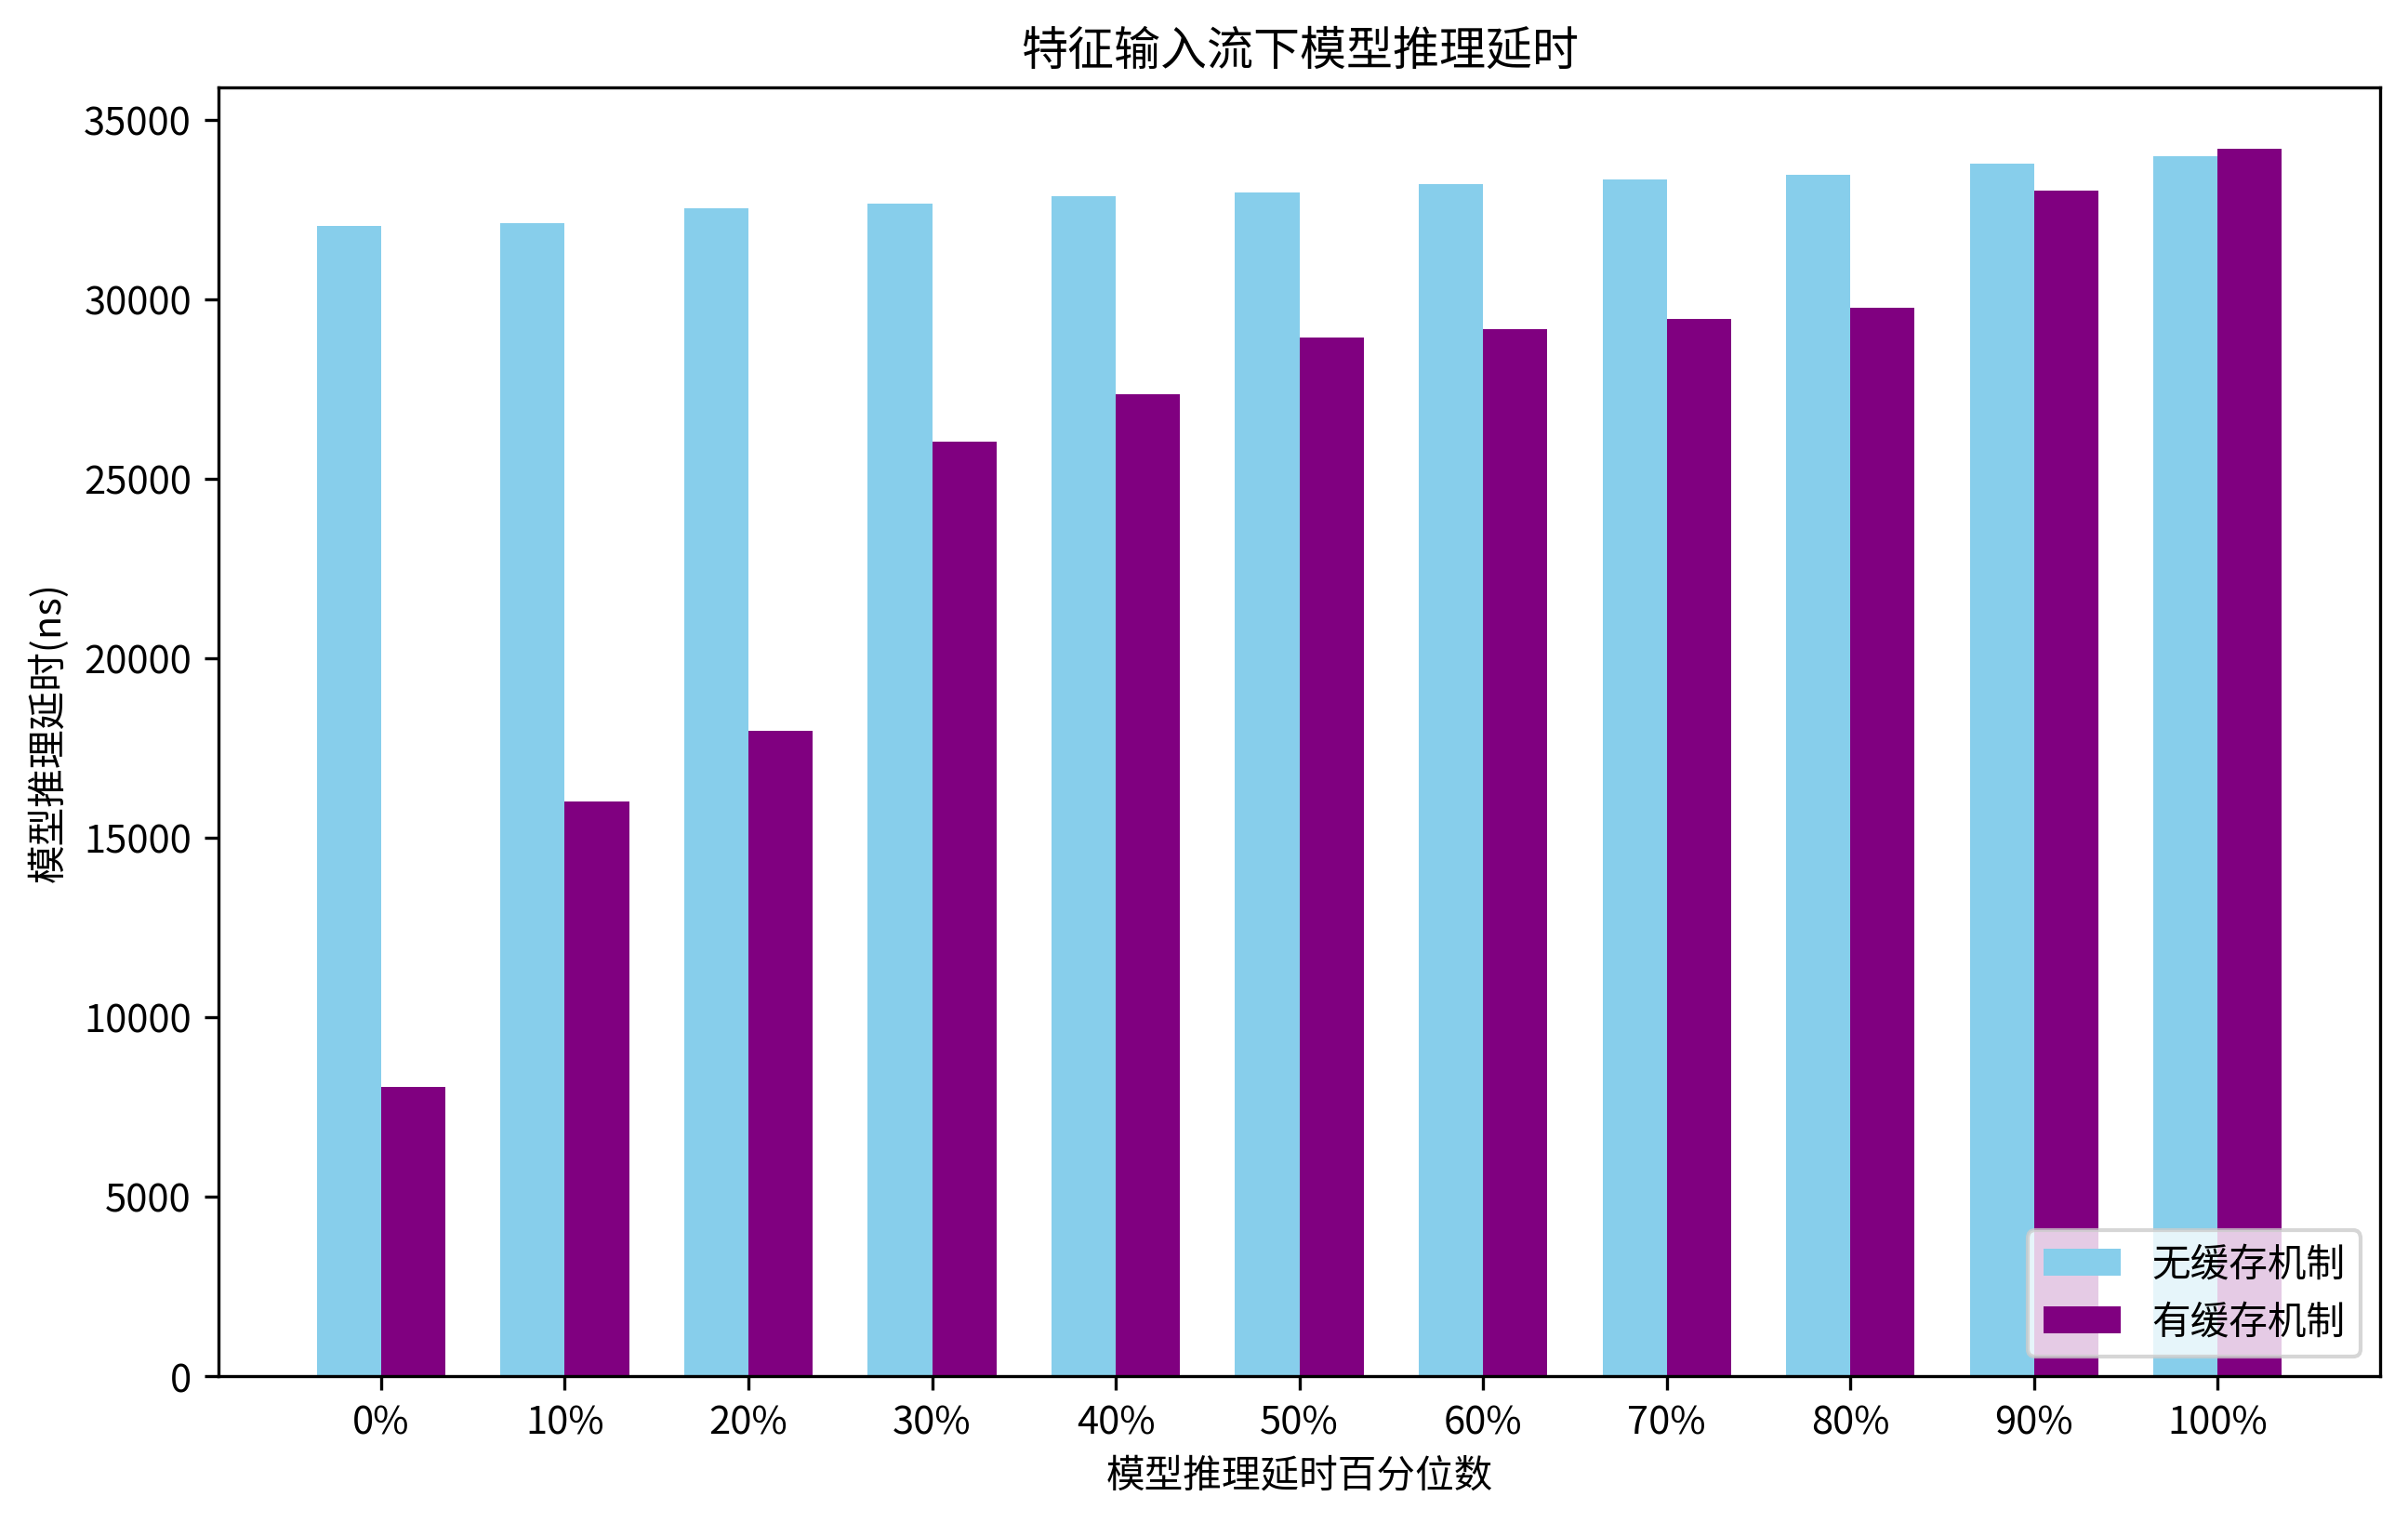
\includegraphics[width=1\textwidth]{image/chap04/outstime.png}
    \caption{启用与不启用缓存机制下测试样例的延时分布}
    \label{fig:hole}
\end{figure}

如图所示,在最大延时部分,观察到启用缓存机制后的延时与未启用时的延时基本一致,可以验证分支缓存机制本身执行过程的高效。
证明了仅仅通过输入匹配和预计算哈希表查询对于多分支因子模型的整体推理延时没有显著增长。
同时,观察到启用缓存机制在低延时交易系统更新行情后的多数情况下都表现出缓存命中带来的显著加速,尤其是对于连续特征输入一致的情况下,切片输入分支的后续融合分支也将产生命中从而极大减小计算量综合产生更显著的加速效果。

\begin{figure}[h]
    \centering
    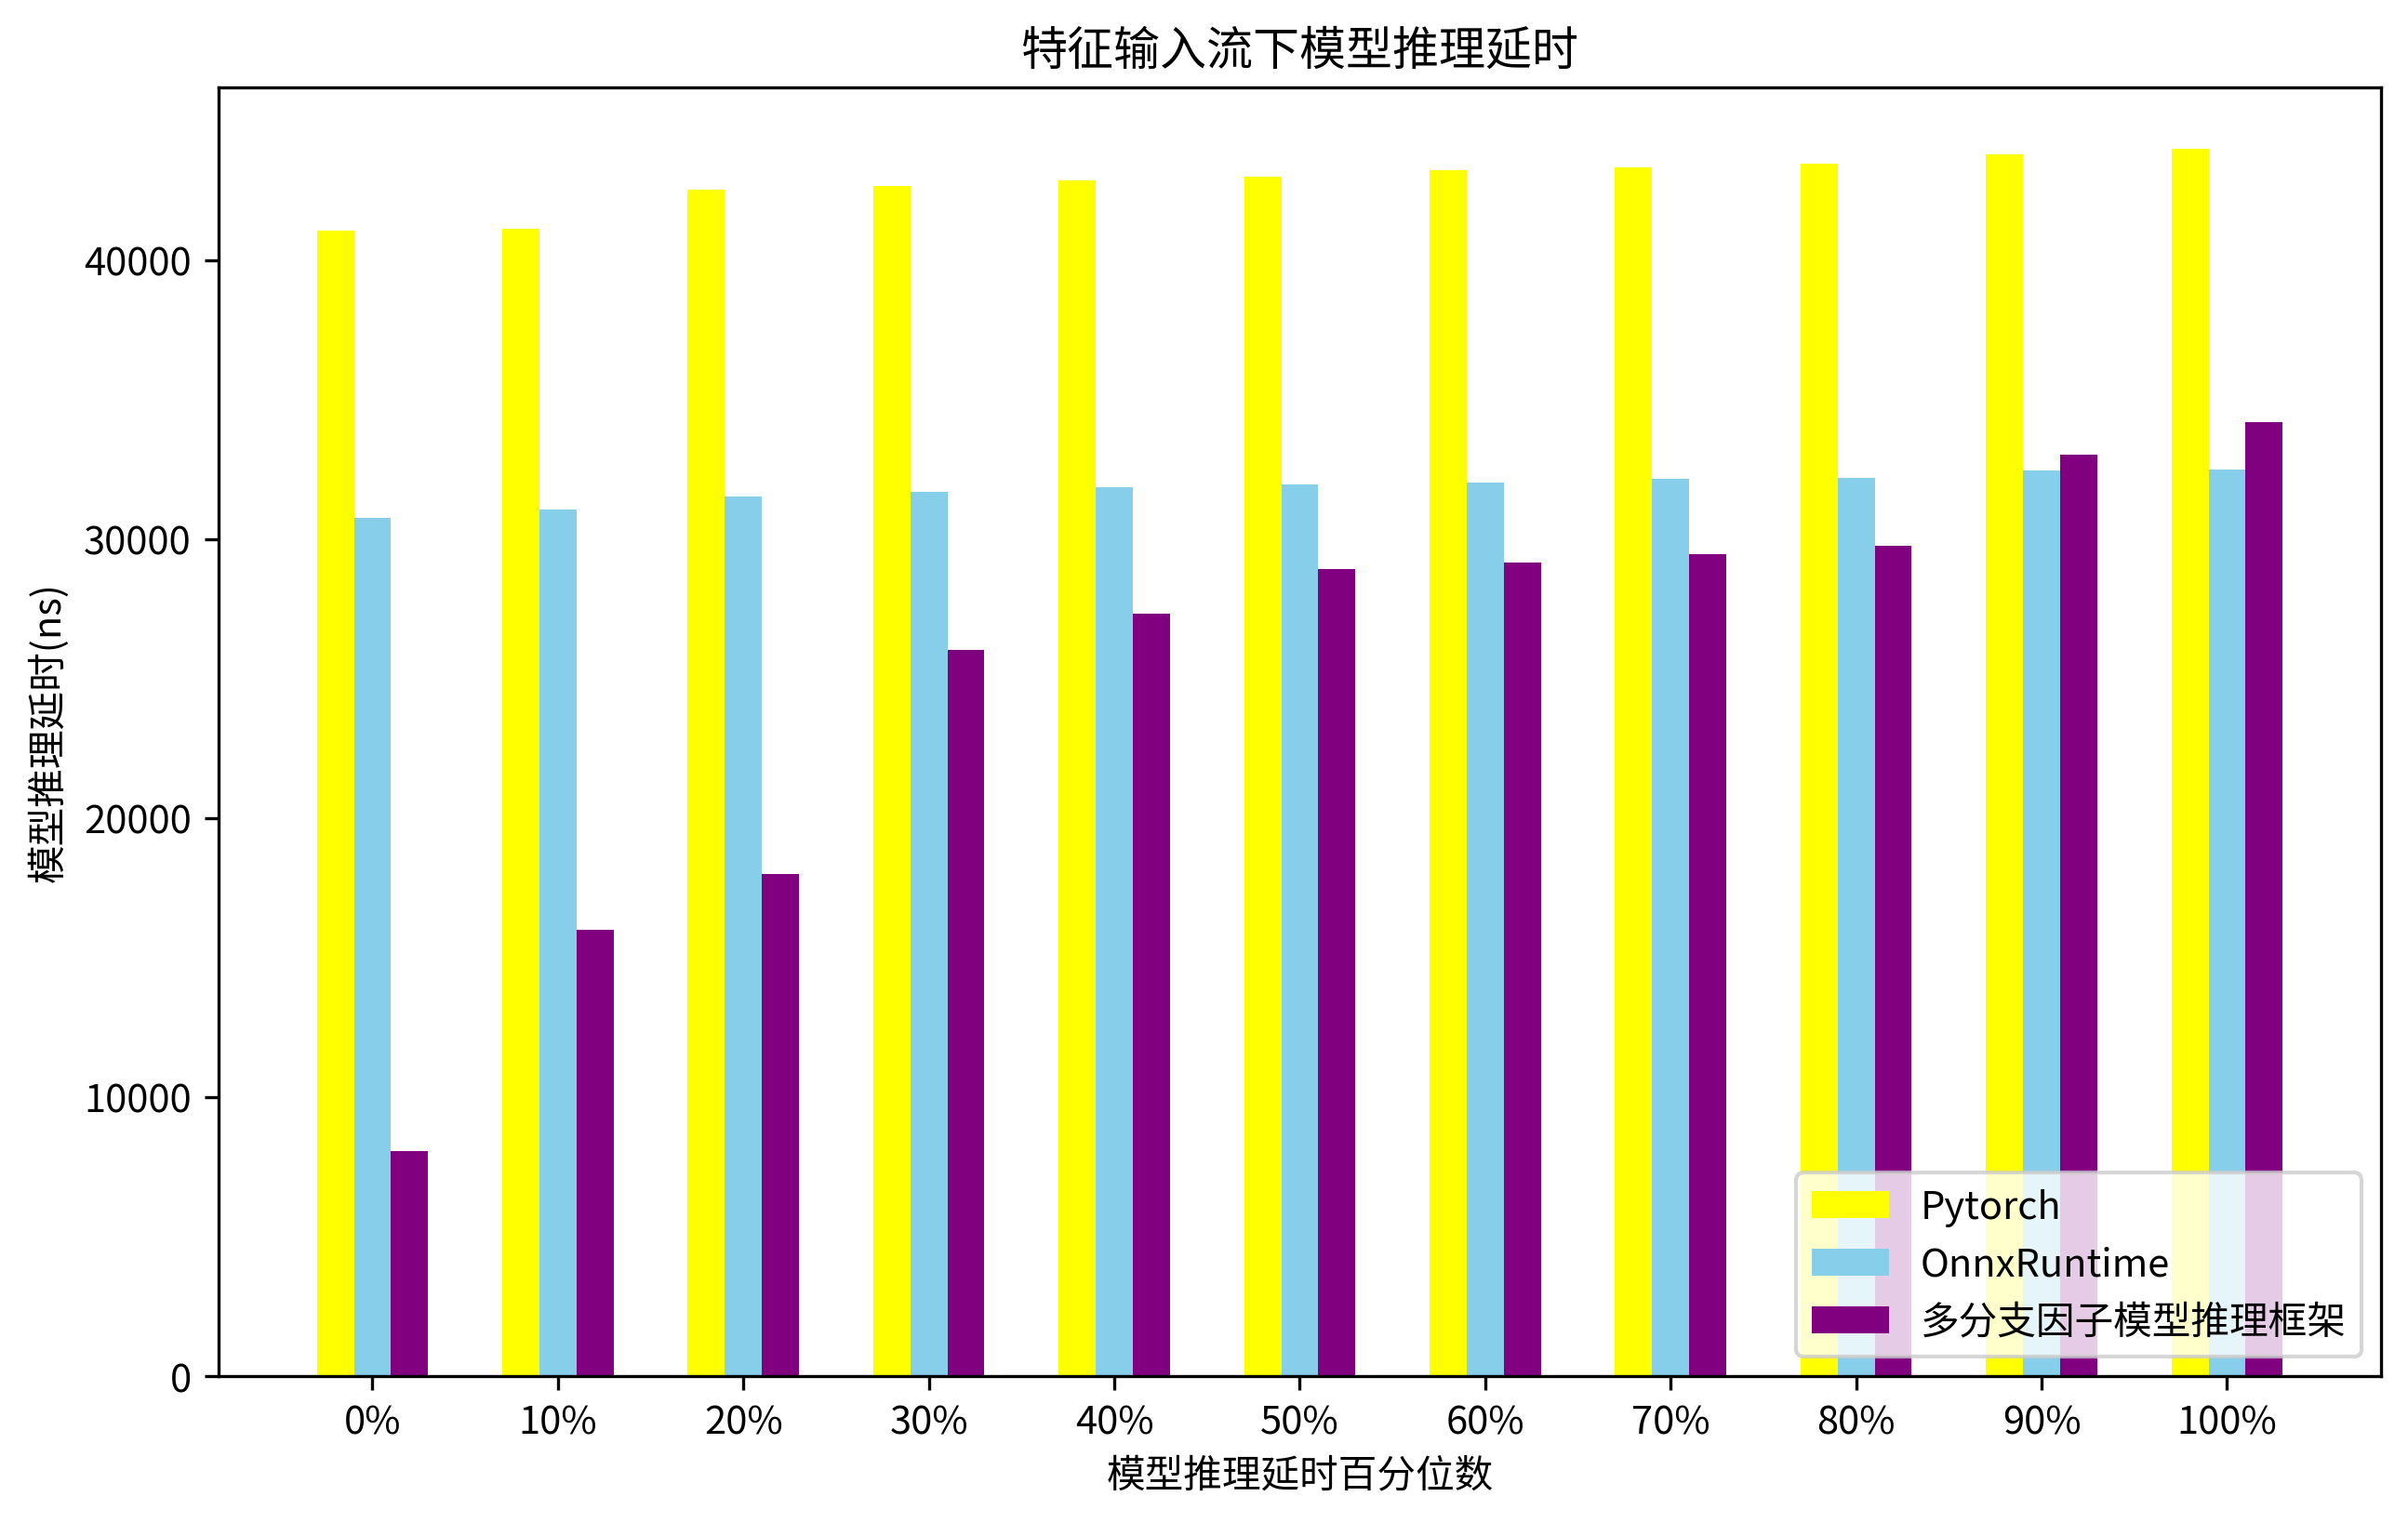
\includegraphics[width=1\textwidth]{image/chap04/outsframe.png}
    \caption{不同推理框架下测试样例的延时分布}
    \label{fig:hole}
\end{figure}

如图所示,在最大延时部分,观察到启用缓存机制后模型推理框架推理延时和Onnx Runtime推理延时显著快于Pytorch JIT。
这代表本文提出的多分支因子模型推理框架作为一个轻量级的专用推理框架本身的基础推理性能较好,这也表现出推理框架在计算图方面静态优化带来的显著性能提升。
同时,尽管在该部分Onnx Runtime推理延时略快于本文提出的多分支因子模型推理框架,但是注意到仅在最大延时部分也就是缓存完全未命中时Onnx Runtime才具有此优势,
因此可以通过在项目中加入输入缓存检查从而在无缓存命中时选择Onnx Runtime推理后端以减小最大延时,从而在最大延时情况下利用Onnx Runtime提高推理效率。

另一方面,注意到在发生缓存命中时,本文提出的多分支因子模型推理框架显著降低了推理延时,实现了从 1.08 倍到 3.82 倍的推理性能提升,相较于Pytorch JIT和Onnx Runtime均具有显著的加速优势。
从而说明分支中的输入匹配和预计算哈希表查询机制在Full Tick行情下具有优越的性能。
